\documentclass{beamer}
\usepackage{tikz}
\usetikzlibrary{arrows.meta,positioning,shapes}
\tikzset{
  onslide/.code args={<#1>#2}{\only<#1>{\pgfkeysalso{#2}}},
  invisible/.style={opacity=0},
  visible on/.style={alt={#1{}{invisible}}},
  alt/.code args={<#1>#2#3}{\alt<#1>{\pgfkeysalso{#2}}{\pgfkeysalso{#3}}},
}
\title{TikZ with overlays}
\author{T. Tikz}
\date{October 2026}
\begin{document}
\begin{frame}\titlepage\end{frame}
\begin{frame}{A growing picture}
  \centering
  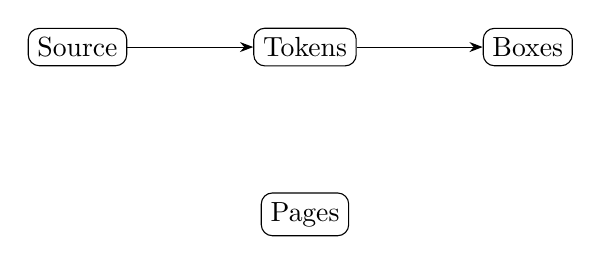
\begin{tikzpicture}[node distance=1.6cm, every node/.style={draw, rounded corners}]
    \node (a) {Source};
    \node (b) [right=of a, visible on=<2->] {Tokens};
    \node (c) [right=of b, visible on=<3->] {Boxes};
    \draw[-Stealth, visible on=<2->] (a) -- (b);
    \draw[-Stealth, visible on=<3->] (b) -- (c);
    \node[onslide=<4>{fill=red!30}, below=of b] {Pages};
  \end{tikzpicture}
\end{frame}
\begin{frame}{Only and pause inside TikZ}
  \begin{tikzpicture}
    \draw[step=0.5, gray!40] (0,0) grid (4,3);
    \only<1>{\fill[blue!40] (0,0) rectangle (1,1);}
    \only<2>{\fill[red!40] (1,1) rectangle (2,2);}
    \pause[3]
    \draw[thick] (0,0) .. controls (1,3) and (3,0) .. (4,3);
  \end{tikzpicture}
\end{frame}
\begin{frame}{Remember picture}
  Point \tikz[remember picture] \node[circle, fill=orange, inner sep=2pt] (p) {};
  here, and an arrow drawn over the page.
  \begin{tikzpicture}[remember picture, overlay]
    \draw<2->[-Stealth, thick, blue] (current page.south west) ++(2,1) -- (p);
    \node<2->[anchor=south east, draw] at (current page.south east) {Overlay};
  \end{tikzpicture}
\end{frame}
\begin{frame}{Shapes and colours}
  
\begin{tikzpicture}
    \foreach \i in {1,...,5} {
      \node<\i->[star, star points=\i+3, fill=blue!\the\numexpr\i*15\relax, minimum size=1cm]
        at (\i*1.5, 0) {};
    }
    \shade[left color=red, right color=yellow] (0,-1.5) rectangle (8,-1);
  \end{tikzpicture}
\end{frame}
\end{document}
